\title{Recap Big data: architectures and data analytics (01QYDOV)}
\author{Jacopo Nasi\\
        Computer Engineer\\
        Politecnico di Torino}
\date{II Period - 2018/2019\\\bigskip\bigskip\today}

\documentclass[12pt]{article}
\usepackage[utf8]{inputenc}
\usepackage[english]{babel}
\usepackage{geometry}
\usepackage{indentfirst} % First line indent
\usepackage{mathtools}
\usepackage{wrapfig}
\usepackage[usenames, dvipsnames]{color}
\usepackage{float}
\usepackage{amssymb}
\usepackage{ifsym}
\usepackage{listings}
\usepackage{multicol}

\usepackage{listings}
\usepackage{color}

\definecolor{dkgreen}{rgb}{0,0.6,0}
\definecolor{gray}{rgb}{0.5,0.5,0.5}
\definecolor{mauve}{rgb}{0.58,0,0.82}

\lstset{frame=tb,
  language=Java,
  aboveskip=3mm,
  belowskip=3mm,
  showstringspaces=false,
  columns=flexible,
  basicstyle={\small\ttfamily},
  numbers=none,
  numberstyle=\tiny\color{gray},
  keywordstyle=\color{blue},
  commentstyle=\color{dkgreen},
  stringstyle=\color{mauve},
  breaklines=true,
  breakatwhitespace=true,
  tabsize=3
}

% Misure Documento
\geometry{ a4paper, total={170mm,257mm},left=35mm, right=35mm, top=35mm, bottom=35mm }

\begin{document}

\begin{figure}
  \centering
  
\includegraphics[width=10cm]{images/polito.pdf}
\end{figure}

\maketitle


\newpage
\tableofcontents

\newpage
{\noindent \Large \textbf{License}\bigskip}

This work is licensed under a Creative Commons Attribution-NonCommercial-ShareAlike 3.0 Unported License.\\
You are free:
\begin{itemize}
  \item \textbf{to Share}: to copy, distribute and transmit the work
  \item \textbf{to Remix}: to adapt the work
\end{itemize}
Under the following conditions:
\begin{itemize}
  \item \textbf{Attribution}: you must attribute the work in the manner specified by the author or licensor (but not in any way that suggests that they endorse you or your use of the work)
  \item \textbf{Noncommercial}: you may not use this work for commercial purposes.
  \item \textbf{Share Alike}: if you alter, transform, or build upon this work, you may distribute the resulting work only under the same or similar license to this one.
\end{itemize}

\noindent More information on the Creative Commons website (http://creativecommons.org).

\begin{figure}[h!]
  \centering
  
\includegraphics[width=3cm]{images/license.png}
\end{figure}

{\noindent \Large \textbf{Acknowledgments}\bigskip}

Questo breve riepilogo non ha alcuno scopo se non quello di agevolare lo studio di me stesso, se vi fosse di aiuto siete liberi di usarlo.\\
Le fonti su cui mi sono basato sono quelle relative al corso offerto (\textbf{Big data: architectures and data analytics (01QYDOV)}) dal Politecnico di Torino durante l'anno accademico 2018/2019.\\
Non mi assumo nessuna responsabilità in merito ad errori o qualsiasi altra cosa. Fatene buon uso!
\newpage

\section{Introduction}
The amount of data increases every days, to analyze them, system must scale according. All these systems must deal with computation capabilities, network bandwidth and failures. A good pratice to solve problems is the parallelizations, a single-node architectiure cannot solve, in reasonable time, the request of these days. For these reasons, nowadays, clusters (fig.\ref{fig:cluster}) are pretty common.
\begin{figure}[H]
  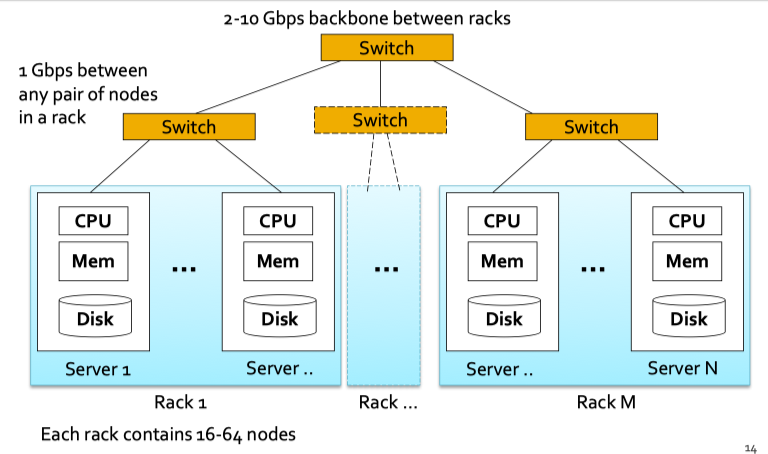
\includegraphics[width=\linewidth]{images/cluster.png}
  \caption{Cluster Architecture}
  \label{fig:cluster}
\end{figure}
The main characteristics are:
\begin{itemize}
  \item \textbf{Scalability}: Increase number of users, amount of datas, complexity of problems
  \begin{itemize}
    \item Scale \textbf{UP}: More power/resources for a single-node
    \item Scale \textbf{OUT}: Add more nodws to the cluster
  \end{itemize}
\end{itemize}

% ==================================================================================
% |                                  APACHE HADOOP                                 |
% ==================================================================================

\section{Apache Hadoop}
Scalable fault-tolerant distributed system for Big Data: Distributed Data Storage, Distributed Data Processing, etc...
Is an Open Source project under Apache license. Is used by a lot of main IT companies all around the world.\\
The core of the structure are:
\begin{itemize}
  \item \textbf{Distributed BD Processing Infrastructure} (MapReduce):
  \begin{itemize}
    \item High-level abstraction view: Not require to take care of scheduling and synchronizations
    \item Fault Tolerant: Node and task are automatically managed
  \end{itemize}
  \item \textbf{HDFS} (Hadoop Distributed File System):
  \begin{itemize}
    \item Fault-Tolerant
    \item High availability distributed storage
  \end{itemize}
\end{itemize}
The paradigm of MapReduce will not be illustrated, in figure \ref{fig:mapreduce} a sample of the process during the word count problem.
\begin{figure}[H]
  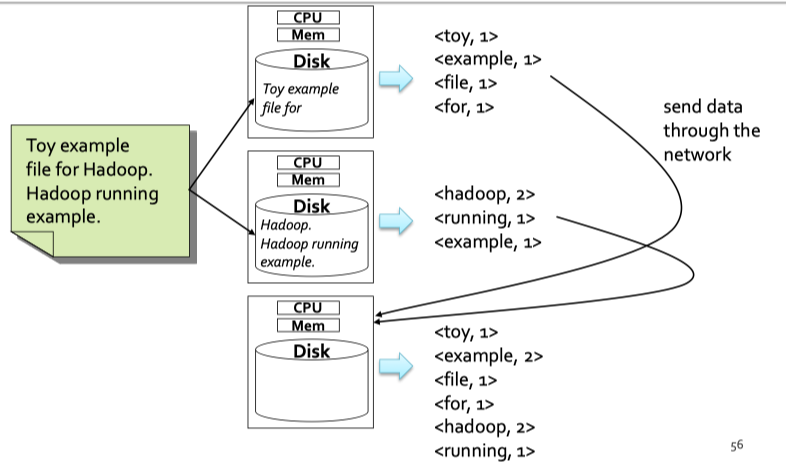
\includegraphics[width=\linewidth]{images/mapreduce.png}
  \caption{MapReduce Example}
  \label{fig:mapreduce}
\end{figure}

\subsection{Structure of a program}
The project is divided in different parts:
\begin{itemize}
  \item Driver: Coordinators of the jobs
  \item Mapper: Class for the Map part
  \item Reducer: Class implementing the Reduce part
\end{itemize}
There are also other important terms:
\begin{itemize}
  \item Job: Execution of a MapReduce code over a dataset
  \item Task: Execution of a Map task or a Reducer task on a slice of data
\end{itemize}
The workflow of a project is similar to the following one:
\begin{figure}[H]
  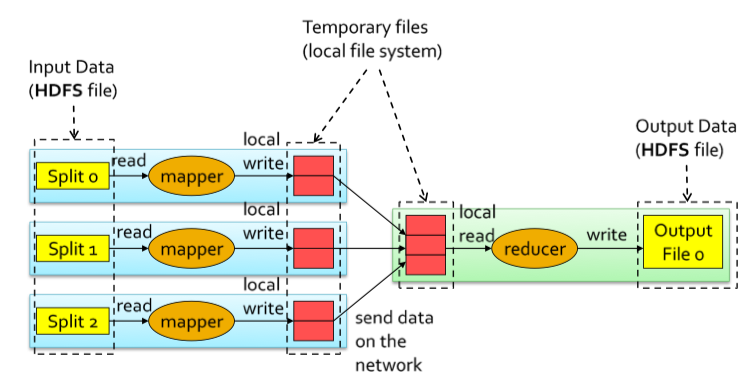
\includegraphics[width=\linewidth]{images/wf.png}
  \caption{MapReduce Workflow in Hadoop}
  \label{fig:wf}
\end{figure}

\subsection{Data Types}
Hadoop make use of its own basic data types:
\begin{itemize}
  \item Text: Like Java string
  \item IntWritable: Like java integer
  \item LongWritable
  \item FloatWritable
\end{itemize}
Also the data for the input and output has its own type:
\begin{itemize}
  \item TextInputFormat (Lines)
  \item KeyValueTextInputFormat (2 Fields)
  \item SequenceFileInputFormat (Binary)
\end{itemize}
Also the output have similar formats.\\
Is also possible to define personalized data types, these also the usage of more complex values. To use them, is required, to implements the \textit{org.apache.hadoop.io.Writable} interface and its methods, in particular:
\begin{itemize}
  \item write()
  \item readFields()
\end{itemize}
also the method toString is important, in order to generate the value to be emit with the pair.

\subsection{Combiner and Counters}
In standard MapReduce applications the (key,value) pairs emitted by mappers are sent to the reducers through the newtork. In some case, a sort of "pre-aggreations" could be useful to improve performances and reduce the amount of data shared on the network.\\
An example with the word count problem with clarify the usage of combiners.
\begin{figure}[H]
  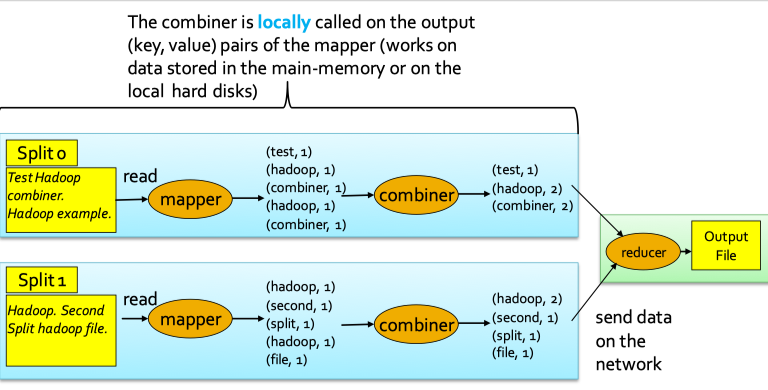
\includegraphics[width=\linewidth]{images/combiners.png}
  \caption{Example of combiner usage}
  \label{fig:cobiners}
\end{figure}
Is an instance of the Reducer class, that implements a pre-reduce phase, characterized by the reduce() method. It process (key, [list of value]) and emits (key, value). It runs on the cluster.\\
Combiners and be also exploited by in-mapper solutions, by initialize a set of in-mapper variables during the instance of the Mapper. They are created by using setup/cleanup methods.\\
Hadoop provides a set of vasic, built-in, counters to store some statistics about jobs, mappers and reducers. Also some ad-hoc, user-defined, counters can be defined. They can be used by the exploting enum Java types, and increment by using the following code:
\begin{lstlisting}
  context.getCounter(countername).increment(value);
\end{lstlisting}

\subsection{Configurations}
Is possible to define some properties shared among the different part (M,C,R), they must be defined in the driver using the following syntax:
\begin{lstlisting}
  conf.set("property-name", "value");
\end{lstlisting}
and they can be retrived in the Mapper and/or Reducer phase by using:
\begin{lstlisting}
  context.getConfiguration().get("property-name");
\end{lstlisting}

\subsection{Map-only job}
In some cases everything can be achived using the Mapper phase only. Of course, Hadoop, allows the execution of this kind of jobs. Everything is achived by setting the number of reducers task to zero. \textbf{Not setting this value can generate problems during the executions}.

\subsection{Setup and Cleanup methods}
Are two optional methods to be invoked in the Mapper class, one at the start (Setup()) and the other at the end, both invoked one time for each mapper.

\subsection{Patterns}
Common patterns to solve problems. The following are know as \textbf{Summarization Patterns}:
\paragraph{Numerical Summarizations} group records/objects by a key filed and calculate a numberical aggregate (avg, min, max, std deviations, etc...). Are used to provide a top-level view of large input data sets. They are used to analyze, by domain experts, trends or anomalies.\\
The phase:
\begin{itemize}
  \item \textbf{Mappers}: Key is used to define groups, Value for computing aggregate statistics
  \item \textbf{Reducers}: Receive a set of numerical values for each "group-by" key and compute the final stats
  \item \textbf{Combiners}: Used to speed-up the process
\end{itemize}

\paragraph{Inverted Index Summarizations} the goal is to build an index from the input data to support faster search or data enrichment.
\begin{itemize}
  \item \textbf{Mappers}: Key is the set of fields to index (a keyword), Value is a unique identifier of the objects to associare with each "keyword"
  \item \textbf{Reducers}: Receive a set of identifiers for each keyword and simply concatenate them
  \item \textbf{Combiners}: Normally NOT used
\end{itemize}

\paragraph{Counting with Counters} the goal is to compute count summarizations of data sets. Also this solutions can be used to identify trends and anomalies.
\begin{itemize}
  \item \textbf{Mappers}: Process each input record and increment a set of counters
\end{itemize}
This pattern can be achived by using also MapOnly jobs, the result are directly printed by the Driver of the application.\\

The following are know as \textbf{Filtering Patterns}:
\paragraph{Filtering} has the goal to filter out input records that are not of interest and keep the others, in order to focusing only on the records of interest. The pourpose is to reduce the set of the data for the analysis.
\begin{itemize}
  \item \textbf{Mappers}: Output one pair for each record that satisfies the enforced rule
  \item \textbf{Reducers}: Almost useless
\end{itemize}

\paragraph{Top K} is select a small set of top K record according to a ranking function. Used to focusing only on the most important (for the ranking function) values.
\begin{itemize}
  \item \textbf{Mappers}: Each mapper initializes an in-mapper top K list (small), cleanup emits the pairs after the complete scan
  \item \textbf{Reducers}: a Single Instance compute the final top k list by merging the local lists
\end{itemize}

\paragraph{Distinct} it finds a unique set of values/records, prune the duplicates.
\begin{itemize}
  \item \textbf{Mappers}: Emit one (key, null) pair for each input record
  \item \textbf{Reducers}: Emit one (key, null) pair for each input (key, [list of values]) pair
\end{itemize}

\subsection{Multiple Inputs/Outputs}
Hadoop allows the user to implements different input and/or outputs, it could be useful in some case. The input differentiation is achieved by using the addInputPath() method, the output one is achieved with addNamedOutput() method.

\subsection{Distributed Cache}
Some application need to share and cache (small) read-only files to performa efficently their tasks. These files should be accessible by all nodes of the cluster in an efficient way. The Distributed Cache is a facility provided by the Hadoop-based MapReduce framework to cache files.
These files are specified in the Driver, during the initialization of the job, Hadoop create a local copy of the shared/cached files in all nodes which are used to execute some tasks of the job, the cache file is then read by the Mapper, usually in the setup method.
Save with:
\begin{lstlisting}
  job.addCacheFile(new Path("hdfsPath").toUri());
\end{lstlisting}
And it is retived by using:
\begin{lstlisting}
  URI[] urisCachedFiles = context.getCacheFiles();
\end{lstlisting}

% Slide set #11
\subsection{Data Organization Patterns}
\paragraph{Shuffling} is a technique used to randomize the order of the data, the motivations are:
\begin{itemize}
  \item Anonymization of data
  \item Selecting a subset of random data
\end{itemize}
The structure is the following:
\begin{itemize}
  \item \textbf{Mappers}: Emit one (key (random), value) pair for each input record
  \item \textbf{Reducers}: Emit one (key, null) pair for each value in [list of values] of the input (key, [list of values]) pair
\end{itemize}

\subsection{Metapatterns}
\paragraph{Job Chaining} is the technique to execute a sequence of jobs (synchornizing them), the intent is to manage workflow of complex applications based on many phases.\\
The driver (single instance) contains the whole workflow and it execute the jobs in the proper order.
\begin{figure}[H]
  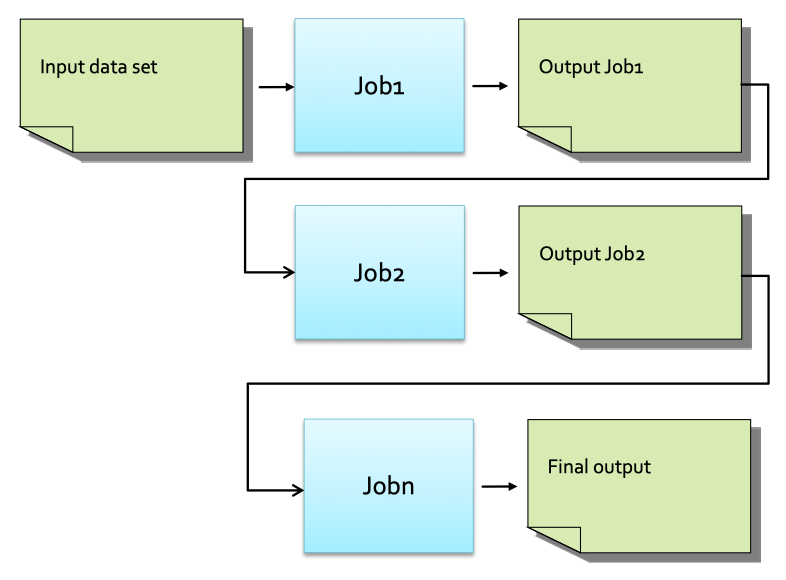
\includegraphics[width=\linewidth]{images/chaining.png}
  \caption{Job Chaining}
  \label{fig:chaining}
\end{figure}

\subsection{Join Patterns}
\paragraph{Reduce side natural join}
The goal is to join the content of two relations (both large), this operation is useful in many applications.\\
Suppose you want to join the following tables:
\begin{itemize}
  \item \textbf{Users}: userid, name, surname
  \item \textbf{Likes}: userid, movieGenre
\end{itemize}
The record of the first table will be:
\begin{center}
  (userid=u1, "Users:name=Paolo,surname=Garza")
\end{center}
While the ones of the second table will be:
\begin{center}
  (userid=u1, "Likes:movieGenre=horror")
  (userid=u1, "Likes:movieGenre=adventure")
\end{center}
The reducers iterate over the values associated with each key (value of the common attributes) and compute the "local natural join" for the current key. The output will be like the followings:
\begin{itemize}
  \item (userid=u1, "Users:name=Paolo,surname=Garza,movieGenre=horror")
  \item (userid=u1, "Users:name=Paolo,surname=Garza,movieGenre=adventure")
\end{itemize}

\paragraph{Map side natural join} the goal is to join the content of the two relations, with a large and a small table (can be loaded in main memory). Is a \textbf{Map-only} job where the mapper process the content of the large table, the distributed cache is used to provide a copy of the small table to all mappers. The process is than a "local natural join" like in the previous pattern.\\
Also the other kind of joins can be achieved.

\subsection{Relational Algebra Operations}
The are a lot of useful operators in the SQL language: \textit{Selection, Projection, Union, Join, Aggregations, Group By, etc...}. The MapReduce paradigm can be used to implement relational operatos, however, the MR implementation is efficient only when a full scan of the input table is needed (selection are better performed by DBMS).\\
Relations/Tables (also the big ones) can be stored in the HDFS distributed file system, they are broken in blocks and spread across the servers of the Hadoop cluster.\\
By definition tables do not contain duplicate records, this constraint must be satisfied by both the input and the output tables.
\paragraph{Selection} only the records that are satisfying a condition can be kept. The schema remain the same. This algebric operation can be achieved by using a filtering pattern.

\paragraph{Projection} it can be achieved by the following structure:
\begin{itemize}
  \item \textbf{Mappers}: For each record select the proper attribute and emits a pair (key=attributeFiltered, value=null)
  \item \textbf{Reducers}: Emit one (key, value) pair for each input with key=attributeFiltered and value=null
\end{itemize}
\paragraph{Union} merge two tables with the same schema, duplicates are removed. Everything can be achieved with the following structure:
\begin{itemize}
  \item \textbf{Mappers}: for each record, of each table, a pair (key=t, null) will be emitted
  \item \textbf{Reducers}: Emit one (key, value) pair for each input (key, [list of values]) pair with key=t and value=null
\end{itemize}

\paragraph{Intersection} using 2 tables with the same schema, produce a third table with the records appearing on both relations.
\begin{itemize}
  \item \textbf{Mappers}: Emit one pair (key=t, value=t) for each record in both relations
  \item \textbf{Reducers}: Emit one (key, value) pair for each input with key=t and value=null for pair containing 2 values.
\end{itemize}

\paragraph{Difference} similar to the previous Intersection, the Reducers, will emit a pair only if its contains 1 value.

\paragraph{Join} can be implemented using the join patterns.

\paragraph{Aggregations and Group By} are implemented by using summarization pattern.

% ==================================================================================
% |                                 APACHE SPARK                                   |
% ==================================================================================
\clearpage
\section{Apache Spark}
\subsection{Introduction}
Apache Spark is a fast and general-pourpose engine for large-scale data rpcoessing. Spark aims at achieving the following goals in the Big Data context:
\begin{itemize}
  \item \textbf{Generality}: Diverse worksload, operators, job size
  \item \textbf{Low Latency}: sub-second
  \item \textbf{Fault Tolerance}: Faults are the norm, not the exception
  \item \textbf{Simplicity}: Often come from generality
\end{itemize}
Iterative jobs, with MapReduce, involve a lot of disk I/O for each iteration and stage, which are slow, even if it is local I/O. The idea behind spark is to reduce the I/O operations by keep more data in main memory. This solutions allow to increase the speed by 10 to 100 times.\\
Data are represented as \textit{Resilient Distributed Datasers (\textbf{RDDs})}, they are partitioned/distributed collections of objects spread across the nodes of a clusters, stored in Main Memory (when it is possible) or on local disk.
Spark programs are written in terms of operations on resilient distributed data sets. The RDDs are built and manipulated through a set of parallel transformations (map, filter, join, etc...) and actions (count, collect, save, etc...). In case of machine failures RDDs are automatically rebuilt. In the following table the difference between Spark and Hadoop:
\begin{figure}[H]
  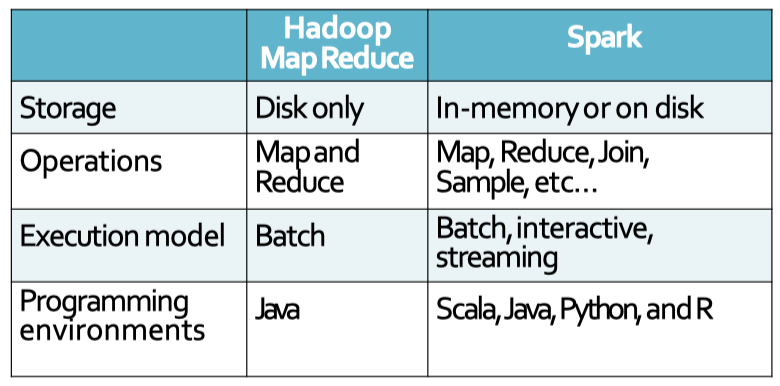
\includegraphics[width=\linewidth]{images/versus.png}
  \caption{MapReduce vs Spark}
  \label{fig:versus}
\end{figure}
\paragraph{Structure} Spark is based on a basic component (the Spark Core) that is exploited by the high-level data analytics components. These provide a more uniform and efficient solution with respect to Hadoop where many non-integrated tools are available. When the efficency of the core component is increased also the efficency of the other high-level components increases.
Th structure contains:
\begin{itemize}
  \item Task scheduling
  \item Memory Management
  \item Fault recovery
\end{itemize}
Spark support also SQL structured datas, also the Hive Query Language.\\
Another important part of Spark is the \textbf{Spark Streaming} real-time, used to process live streams of data in real-time, the APIs used are similar to the one used to process standard and static resources.\\
\textbf{MLlib} is a machine learning/data mining library, it can be used to apply the parallel versions of some ML/DM algorithms (data pre-processing and dimensional reduction, classification algorithms, clustering, itemset mining, etc...).\\
\textbf{GraphX} is a grap processing library, it provides many algorithms for manipulating graphs:
\begin{itemize}
  \item Subgraph searching
  \item PageRank
\end{itemize}
Spark can exploit many \textbf{Schedulers} to execute its applications:
\begin{itemize}
  \item Hadoop YARN
  \item Mesos cluster
  \item Standalone Spark Scheduler
\end{itemize}

\subsection{Basic Concepts}
RDDs are the primary abstraction in Spark, are distributed collections of objects spread across the nodes of a clusters. They are split in partitions, each node of the cluster that is running an application contains at least one partition of the RDDs that is (are) defined in the application. RDDs are store in the main memory of executors running in the nodes of the cluster, when is possible, or in the local disk of the nodes if there is not enough main memory. This type of data allows execution in parallel, of the code, invoked on them. Are also immutable once constructed. Spark tracks lineage information to efficiently recompute lost data (due to failures).\\
RDDs can be created:
\begin{itemize}
  \item By parallelizing existing collections of the hosting programming language
  \item From large files stored in HDFS
  \item From files stored in many traditional file systems or databases
  \item By transforming an existing RDDs
\end{itemize}

\paragraph{Software structure} everything start from the main method, that defines the workflow of the application. The accesses to Spark is made available through the SparkContext object (a connection to the cluster). After the allocation of RDDs it invokes parallel operations over them.
\begin{figure}[H]
  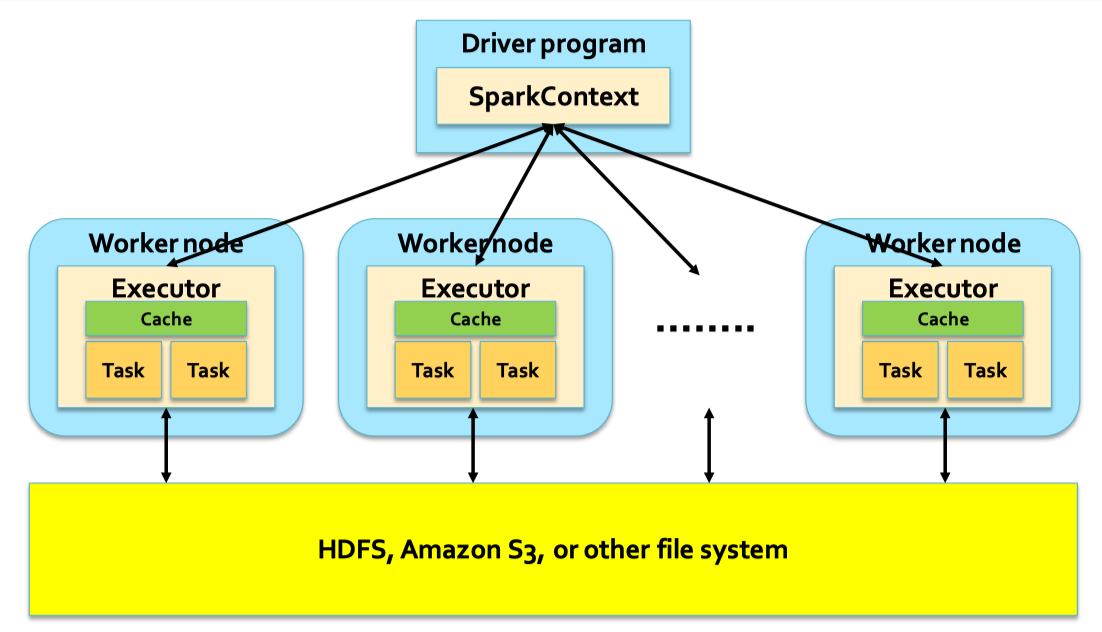
\includegraphics[width=\linewidth]{images/execution.png}
  \caption{Distributed execution of Spark}
  \label{fig:execution}
\end{figure}

\paragraph{Terminology} defined by Spark:
\begin{itemize}
  \item \textbf{Application}: User program built on Spark (Driver, Executors)
  \item \textbf{Application JAR}: A Jar containing the user's Spark application
  \item \textbf{Driver Program}: The process running the main() function of the application and creating the SparkContext
  \item \textbf{Cluster Manager}: An external service for acquiring resources on the cluster
  \item \textbf{Deploy Mode}: Distinguishes where the driver process runs in CLUSTER or CLIENT mode
  \item \textbf{Worker Node}: Any node of the cluster that can run application code in the cluster
  \item \textbf{Executor}: A process launched for an application on a worker node, that runs tasks and keeps data in memory or disk storage across them
  \item \textbf{Task}: A unit of work that will be sent to one executor
  \item \textbf{Job}: A parallel computation consisting of multiple tasks that gets spawned in response to a Spark action
  \item \textbf{Stage}: Each job gets divided into smaller sets of tasks called stages that depend on each other
\end{itemize}

\subsection{RDD-based Programming}
The SparkContext is the connection of the driver to the cluster, is build by means of the constructor of JavaSparkContext. Example:
\begin{lstlisting}
  SparkConf conf = new SparkConf().setAppName("Application name");
  JavaSparkContext sc = new JavaSparkContext(conf);
\end{lstlisting}
\paragraph{RDD} are immutable distributed collection of objects, each split in partitions, this choice allows parallelizing the code based on RDDs. THey can contain any type of Scala, Java and Python Objects.\\
The \textbf{creation} of an RDDs can be achieved in 2 ways:
\begin{itemize}
  \item Loading an external dataset: content of a folder, signle file, database table, etc.
  \item Parallelizing a local collection of objects created in the driver
\end{itemize}
An RDD can be build from an input textual file. It is based on the textFile() method of the JavaSparkContext class. The created RDD is an RDD of Strings, each line of the input file is associated with an object of created RDD. If the input file is an HDFS file, the number of partitions of RDD, is equal to the number of HDFS block used to store the file. Partitions can be also defined manually.\\
Is possible to build RDD from a local Java Objects by using the parallelize method of the JavaSparkContext.\\
\textbf{Saving} RDDs can be easily achieved by store them in a textual (HDFS) file by using the method saveAsTextFile() of the JavaRDD class.\\
The content of RDDs can be retrived from the nodes of the cluster and "stored" in a local Java variable of the Driver, is important to pay attention to the size of the RDD.
\paragraph{Operations} there are two types of supported operations:
\begin{itemize}
  \item Transformations
  \item Actions
\end{itemize}
The \textbf{transformations} are operations on RDDs that return a new RDD. They apply a transformation on the elements of the input and the result of the transformation is "stored in/associated to" a new RDD (they are immutable). They are computed lazily, only when action is applied on the RDDs generated by the transformation operations. Spark keeps track of the dependency between the input RDD and the new RDD returned by the transformation. This graph of depencencies between RDDs represents the information about which RDDs are used to create a new RDD; this is called \textbf{lineage graph} and is represented as a DAG (Direct Acyclic Graph). The graph is also useful for optimization purposes.\\
The \textbf{actions} are operations that return results to the driver program or write the result in the storage.
\paragraph{Functions to Transformations and Actions} Many transformations and some actions are based on user provided functions that specify which "transformation" function must be applied on each element of the input RDD. For example the filter() trans. selects the elements of an RDD satisfying a user specified constraint. The passing can be achieved in different ways in relations to the language, in Java is performed by passing objects of the classes that implement one of the Spark's function interfaces. The interfaces are many, here some of them:
\begin{figure}[H]
  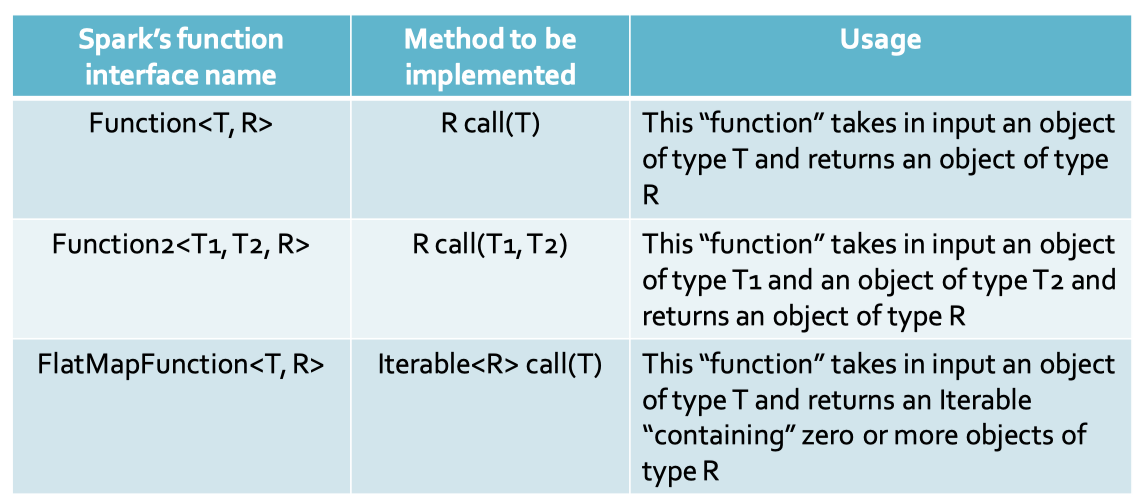
\includegraphics[width=\linewidth]{images/interface.png}
  \caption{Spark function interfaces}
  \label{fig:interface}
\end{figure}
Lambdas function can be useful.
\paragraph{Basic Transformations} some of them analyze the content of one single RDD and return a new RDD:
\begin{itemize}
  \item Filter \item Map \item flatMap \item Distinct \item Sample
\end{itemize}
Some others trans. analyze the content of two input RDDs and return a new one:
\begin{itemize}
  \item Union \item Intersection \item Subtract \item Cartesian
\end{itemize}
\paragraph{Filter()} is the name suggests, is a transformations used to get a new RDD with elements that are satisfying the condition proposed. Example: \textit{Only lines containing word: "error"}.
\paragraph{Map()} method used to compute a function over the whole data contained in the RDD. Example: \textit{Creating an RDDs containing the length of each surname}. The returned RDD contains an element for each of the RDD of input. \paragraph{FlatMap()} is similar to Map(), but a set of elements (0-many) is returned. Example: \textit{input element x, the set of elements with values from x to 3 are returned}.
\paragraph{Distinct()} applied on one single RDD and return a new RDD containing the list of distinct elements of the input RDD. Is an expensive operation.
\paragraph{Sample()} it create a new RDD containing a random sample of the elements of the input RDD.\\
These were all the transformations based on a single RDD. The following make use of 2 input RDDs and they are returning one only.
\paragraph{Union()} it merge two RDDs, but \textbf{without} removing duplicates (can be achieved by passing RDD obtained by the union() to distinct()).
\paragraph{Subtract()} generate an RDD which contains the elements appearing only in the RDD on which the subtract method is invoked and not in the RDD passed as parameter.
\paragraph{Cartesian()} can be applied on RDDs of different data type, the return RDD is an RDD of pairs (JavaPairRDD) containing all the combinations composed on one element of the first input RDD and the second input RDD.

\subsection{DoubleRDDs and statistical measures}
Spark provides specific actions for a specific numerical type of RDD called JavaDoubleRDD, they are different from the euqivalent JavaRDD<type>. The following actions are available: \textit{sum()}, \textit{mean()}, \textit{stdev()}, \textit{variance()}, \textit{max()}, \textit{min()}, etc... A generic JavaRDD$<$T$>$ containing elements of type T can be transformed in a JavaDouble RDD by using two specific transformations: \textit{mapToDouble} or \textit{flatMapToDouble}. They operate similarly to map and flatMap, but they return a JavaDoubleRDD. Ca be also directly generated by the JavaSparkContext.
\paragraph{MapToDouble} the goal is to create a DoubleRDD by applying a function on each element of the input RDD. An example could be: \textit{Create an RDD from a textual file containing the surnames of a list of users and a DOubleRDD containing the lengths of the input surnames}. Also the \textbf{flatMapToDouble} has a similar behaviour.
\paragraph{Actions} the following are applicable only on JavaDoubleRDDs and return a Double value: \textit{sum()}, \textit{mean()}, \textit{stdev()}, \textit{variance()}, \textit{max()}, \textit{min()}. Applying these functions to the objects containing {1.5, 3.5, 2.0} will give the results showed in the following table:
\begin{figure}[H]
  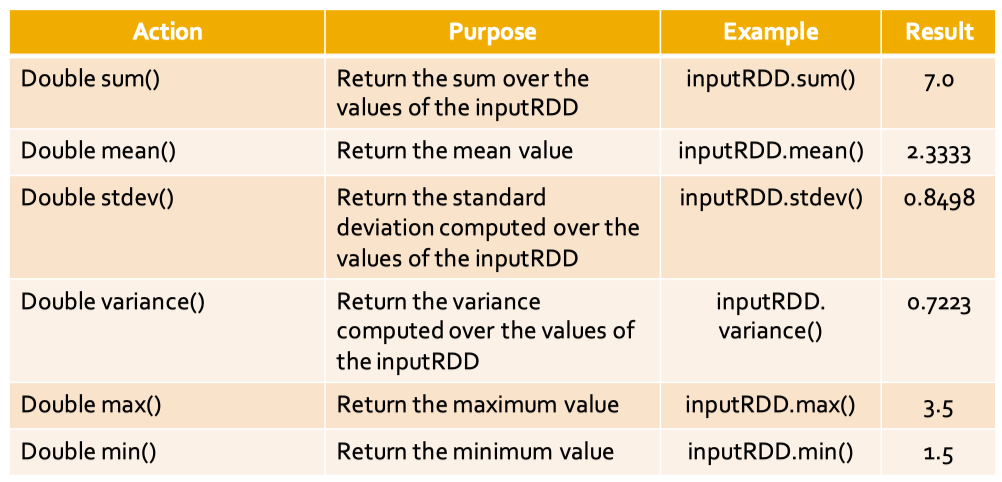
\includegraphics[width=\linewidth]{images/DoubleActions.png}
  \caption{Double Actions}
  \label{fig:DoubleActions}
\end{figure}

\subsection{Cache, Accumulators and Broadcast variables}
\paragraph{Persistence and Cache} spark compute the content of an RDD each time an action is invoked on it. If the same RDD is used multiple times in an application, it recomputes its content every time an action is invoked on the the RDD, or on one of its descendants, this is really expensive, especially for iterative applications. Spark allows to make persistent/cache RDDs.\\
When you ask Spark to persist/cache an RDD, each node stores the content of any partitions of it that it computes in memory and reuses them in other actions on that dataset. The first time the content of a persistent/cached RDD is computed in an action, it will be kept in memory on the nodes, the next actions on the same RDD will read its content from memory.\\
Spark supports several storage levels, they are used to specify if the content of the RDD is stored:
\begin{itemize}
  \item In the main memory of the nodes
  \item On the local disks of the nodes
  \item Partially in the main memory and partially on disk
\end{itemize}
To create a persistent RDD is enough to use the method \textit{persist()} by passing the storage level. Using the \textit{StorageLevel.MEMORY\_ONLY()} is equivalent to invoke directly the method \textit{cache()} on the RDD.\\
Storing the RDDs on disk is useful only if:
\begin{itemize}
  \item The size of the RDD is significantly smaller than the size of the input dataset
  \item The functions that are used to compute the content of the RDD are expensive
  \item Recoumputing a partition may be as fast as reading it from disk
\end{itemize}
To remove data from the cache is enough to invoke the method \textit{unpersist()}.

\paragraph{Accumulators} when a function passed to a Spark operation is executed on a remote cluster node, it works on separate copies of all the variables used in the function. These variables are copied to each node of the cluster, and no updates to the variables on the nodes are propagatetd back to the driver program. Spark provides a type of shared variables called accumulators, they are shared variables that are only "added" to through an associative operation and can therefore be efficiently supported in parallel, they can also be used to implement counters (as in MapReduce) or sums.\\
\textbf{Accumulators are usually used to compute simple statistics} while performing some other actions on the input RDD. THe driver defines adn initializes the accumulator, the code executed in the worker nodes increases the value of the accumulator. The final value of the accumulator is returned to the driver node, that is the only one with the correct rights to access to the final value. The value of the accumulator is increased in the call method of the functions associated with transformations. Since transforations are lazily evaluated, the value of the accumulator is computed only when an action is executed on the RDD on which the transformations increasing the accumlator are applied. Natively Long and Double are supported, others can be added by developers. Here an example of the usage of the accumulators:
\begin{lstlisting}
  // Define an accumulator of type long
  final LongAccumulator invalidEmails = sc.sc().longAccumulator();

  // Read the content of the input textual file
  JavaRDD<String> emailsRDD = sc.textFile("emails.txt");

  // Select only valid emails
  JavaRDD<String> validEmailsRDD = emailsRDD.filter(line -> {
    // Increase the accumulator if the line contains an invalid email
    if (line.contains("@")==false)
      invalidEmails.add(1);
    return line.contains("@");
  });
\end{lstlisting}

\paragraph{Broadcast variables} also these are supported by Spark. They are read-only (medium/large) shared variable, they are instantiated in the driver and they are sent to all worker nodes that use it in one or more Spark actions. They are usually used to share large lookup-tables.\\
An example: \textit{Create an RDD from a textual file containing a dictionary of pairs (word, integer)} the code will be the following:
\begin{lstlisting}
  // Read the content of the dictionary from the first file and
  // map each line to a pair (word, integer value)
  JavaPairRDD<String, Integer> dictionaryRDD = sc.textFile("dictionary.txt").mapToPair(line ->
    {
      String[] fields = line.split(" ");
      String word=fields[0];
      Integer intWord=Integer.parseInt(fields[1]);
      return new Tuple2<String, Integer>(word, intWord) ;
    });

  // Create a local HashMap object that will be used to store the
  // mapping word -> integer
  HashMap<String, Integer> dictionary=new HashMap<String, Integer>();

  // Create a broadcast variable based on the content of dictionaryRDD
  // Pay attention that a broadcast variable can be instantiated only
  // by passing as parameter a local java variable and not an RDD.
  // Hence, the collect method is used to retrieve the content of the
  // RDD and store it in the dictionary HashMap<String, Integer> variable
  for (Tuple2<String, Integer> pair: dictionaryRDD.collect()) {
    dictionary.put(pair._1(), pair._2());
  }

  final Broadcast<HashMap<String, Integer>> dictionaryBroadcast = sc.broadcast(dictionary);
\end{lstlisting}

\end{document}
